%\documentclass[aps, prl, preprint]{revtex4-1}
\documentclass{article}
\usepackage{amsmath}
\usepackage{amsthm}
\usepackage{amsfonts}
\usepackage{amssymb}
\usepackage{courier}
\usepackage{graphicx}
\usepackage{physics}
\usepackage{mathrsfs}
\usepackage{geometry}
\usepackage{hyperref}

\hypersetup{colorlinks = true, urlcolor = blue}
\geometry{margin=1in}

\newcommand{\ten}{\otimes}
\newcommand{\Tra}[1]{\Tr\left\{#1\right\}}
\newcommand{\Ptra}[2]{\Tr_{#1}\left\{#2\right\}}
\newcommand{\til}[1]{\widetilde{#1}}
\newcommand{\ave}[2]{\langle #1\rangle_{#2}}
\newcommand{\I}{\mathcal{I}}

\begin{document}

%% RevTeX 4.1 Title Setup

%\title{Notes on the Born-Markov Master Equations}
%\author{Garrett Higginbotham}
%\email{ghiggie@uab.edu}
%\affiliation{Department of Physics\\The University of Alabama at Birmingham}
%\date{\today}
%\begin{abstract}
%We derive the Born-Markov equations, with and without the secular approximation.
%\end{abstract}

%% Regular Title Setup

\title{Notes on the Born-Markov Master Equations}
\author{Garrett Higginbotham\\ghiggie@uab.edu\\Department of Physics\\The University of Alabama at Birmingham}

\maketitle
\tableofcontents

\section{Closed Systems Formalism}

\subsection{Setup}

For all calculations, we use a unit system in which $\hbar = 1$. Consider a bipartite system consisting of subsystems $A$ and $B$, each of which are possibly multipartite. We write the Hamiltonian of the entire system as
\begin{equation}\label{ham}
H_{AB} = H_0 + V_I
\end{equation}
where $H_0 =  (H_A+V_A)\ten\I_B + \I_A\ten (H_B+V_B)$ is the free Hamiltonian for systems $A$ and $B$, and where $V_I$ mediates the shared behavior between the systems. For now we will only consider the case in which the total Hamiltonian is time-independent, reserving the time-dependent case for a later analysis.

We assume that the systems $A$ and $B$, when taken together, form a closed system. In this case, the state of the system evolves under standard von Neumann evolution:
\begin{equation}\label{vnAB}
\dot{\rho}_{AB}(t) = -i\comm{H_{AB}}{\rho_{AB}(t)}
\end{equation}
Here, $\rho_{AB}$ is the density operator describing the state of the closed system. It is expected that any such density operator must satisfy the following conditions:
\begin{enumerate}
	\item Hermiticity: $\rho = \rho^{\dag}$
	\item Positivity: $\rho \geq 0$ (i.e., $\forall \lambda\in \text{Spec}(\rho),\ \lambda \geq 0$)
	\item Normalization: $\Tra{\rho} = 1$
\end{enumerate}
These properties are required in order to ensure that the density operator gives rise to proper statistical distributions. The first condition ensures that the probabilities are real numbers, the second ensures that the probabilities are non-negative, and the final condition ensures that the probabilities sum to $1$.

\subsection{Interaction Picture}

We will now switch from the Schr{\"o}dinger picture to the interaction picture by introducing the invertible mapping
\begin{equation}\label{intpic}
\til{A}(t) = e^{iH_0t}Ae^{-iH_0t}
\end{equation}
where $A$ is an arbitrary operator in the Schr{\"o}dinger picture, and $\til{A}(t)$ is the corresponding operator in the interaction picture. It is stressed that $\til{A}(t)$ is usually time-dependent, even if $A$ is time-independent. An example of them both being time-independent occurs when $\comm{A}{H_0} = 0$, in which case $\til{A}(t) = A$. Further, note that $\til{A}(0) = A$ is always true. In the interaction picture, the von Neumann equation is given by
\begin{equation}\label{intdyn}
\dv{t}\til{\rho}_{AB}(t) = -i\comm{\til{V}_I(t)}{\til{\rho}_{AB}(t)}
\end{equation}
Switching from the Schr{\"o}dinger picture to the interaction picture has the effect of removing the free Hamiltonians from the dynamics, allowing us to focus our attention on the interaction between systems $A$ and $B$. Equation~\ref{intdyn} may be formally integrated to give
\begin{equation}\label{tmp}
\til{\rho}_{AB}(t) = \til{\rho}_{AB}(0) + (-i)\int_0^{t}\dd{t_1}\comm{\til{V}_I(t_1)}{\til{\rho}_{AB}(t_1)}
\end{equation}
Unfortunately, the right hand side of equation~\ref{tmp} still contains $\til{\rho}_{AB}(t)$ at an intermediate time value, so it isn't particularly useful. However, we may substitute equation~\ref{tmp} into equation~\ref{intdyn} to obtain
\begin{equation}\label{totintpert}
\dv{t}\til{\rho}_{AB}(t) = (-i)\comm{\til{V_I}(t)}{\til{\rho}_{AB}(0)} + (-i)^2\int_0^{t}\dd{t_1}\comm{\til{V_I}(t)}{\comm{\til{V}_I(t_1)}{\til{\rho}_{AB}(t_1)}}.
\end{equation}
This will serve as the starting point for our upcoming approximations.

\section{Open Formalism from Closed Formalism}

Our goal is to try to extract information regarding system $A$ while ignoring system $B$. Physically, this may simply be because system $B$ has too many degrees of freedom to be feasibly studied, such as the case of an atom coupled to a thermal reservoir. In order to quantify the known information regarding the subsystem $A$, we want to create a density operator $\rho_A$ from the operator $\rho_{AB}$. The map $\rho_{AB}\mapsto\rho_A$ is given by the expression
\begin{equation}\label{ptra}
\rho_A = \Ptra{A}{\rho_{AB}}\equiv\sum_{\beta}\qty(\I\ten\bra{\beta})\rho_{AB}\qty(\I\ten\ket{\beta})
\end{equation}
where $\{\ket{\beta}\}$ is an orthonormal basis of system $B$. This mapping is called the \textit{partial trace}, taken with respect to system $B$. It can be shown that this mapping is the \textit{unique} mapping that satisfies the three density operator conditions (for a nice proof of this statement, see Box $2.6$ in Nielsen and Chuang, \textit{Quantum Computation and Quantum Information}).

BRIEFLY DISCUSS THE PROPERTIES OF PARTIAL TRACE
\begin{enumerate}
	\item $\Ptra{A}{\Ptra{B}{\rho_{AB}}} = \Ptra{B}{\Ptra{A}{\rho_{AB}}} = \Tra{\rho_{AB}}$
\end{enumerate}

We will now apply the partial trace to the von Neumann evolution in the interaction picture in an attempt to derive the dynamics for $\til{\rho}_A(t)$. It can be shown (see Appendix) that the order of applying partial trace and interaction picture is irrelevant, so that we can safely obtain the correct dynamics by first computing the interaction picture density operator and then applying the partial trace, instead of going the other direction. Applying partial trace, we obtain
\begin{equation}\label{partintpert}
\dv{t}\Ptra{B}{\til{\rho}_{AB}(t)} = (-i)\Ptra{B}{\comm{\til{V_I}(t)}{\til{\rho}_{AB}(0)}} + (-i)^2\int_0^{t}\dd{t_1}\Ptra{B}{\comm{\til{V_I}(t)}{\comm{\til{V}_I(t_1)}{\til{\rho}_{AB}(t_1)}}}.
\end{equation}
Everything to this point has been exact, and we are ready to begin making assumptions and approximations about the model.

\section{Approximations}

Before we move further, we make the assumption that the inter-system interaction $V_I$ takes on a bilinear form
\begin{equation}\label{coup}
V_I = \sum_{\alpha} A_{\alpha}\ten X_{\alpha}
\end{equation}
Although we require that $V_I$ be Hermitian, we do not necessarily require that $A_{\alpha}$ and $X_{\alpha}$ be Hermitian. We simply require that if $A_{\alpha}\ten X_{\alpha}$ is in the summation, then there exists an index $\beta$ such that $A_{\beta}^{\dag}\ten X_{\beta}^{\dag}$ is also in the summation (for example, consider $V_I = \sigma^{\dag}\ten X + \sigma\ten X^{\dag}$, where $\sigma$ and $X$ are not necessarily Hermitian). With this setup, we write
\begin{equation}\label{coupdag}
V_I^{\dag} = \sum_{\beta} A_{\beta}^{\dag}\ten X_{\beta}^{\dag} = V_I
\end{equation}
We will use equation~\ref{coup} for $\til{V}_I(t)$ and equation~\ref{coupdag} for $\til{V}_I(t_1)$. (We should explicitly compute the interaction picture versions of $\til{V}_I$, but it should also be trivial.) Substituting these into equation~\ref{partintpert}, we obtain
\begin{align}\label{ugh}
\begin{split}
\dv{t}\Ptra{B}{\til{\rho}_{AB}(t)} &= (-i)\sum_{\alpha}\Ptra{B}{\comm{\til{A}_{\alpha}(t)\ten\til{X}_{\alpha}(t)}{\til{\rho}_{AB}(0)}}\\
&+ (-i)^2\sum_{\alpha,\beta}\int_0^{t}\dd{t_1}\Ptra{B}{\comm{\til{A}_{\alpha}(t)\ten\til{X}_{\alpha}(t)}{\comm{\til{A}^{\dag}_{\beta}(t_1)\ten\til{X}_{\beta}^{\dag}(t_1)}{\til{\rho}_{AB}(t_1)}}}
\end{split}
\end{align}

\subsection{Born Approximation}

We assume that system $B$ has many, many more degrees of freedom than system $A$, and we further assume that system $B$ is initially in a Gibbs state $\rho_B^G$, so that the initial state of the system is $\rho_{AB}(0) = \rho_A(0)\ten\rho_B^G$. During the course of the total evolution, system $B$ will cause changes in system $A$, and system $A$ will likewise cause changes in system $B$. However, because system $B$ has so many degrees of freedom, system $B$ will quickly relax to another Gibbs state, thus staying in a Gibbs state for all perceivable time (this is the typicality argument). Because we assume that the systems are weakly coupled, we may make the Born approximation
\begin{equation}\label{born}
\rho_{AB}(t) = \rho_A(t)\ten\rho_B(t) + \rho_{corr}(t)\approx \rho_A(t)\ten\rho_B^G
\end{equation}
Substituting \ref{born} into \ref{ugh} and expanding the Kronecker products and partial traces, we obtain
\begin{align}\label{fuckmyass}
\begin{split}
\dv{t}\til{\rho}_A(t) &= (-i)\sum_{\alpha}\comm{\til{A}_{\alpha}(t)}{\til{\rho}_A(t)}\ave{\til{X}_{\alpha}(t)}{\rho_B^G}\\
&+ (-i)^2\sum_{\alpha,\beta}\int_0^t\dd{t_1}\left\{\comm{\til{A}_{\alpha}(t)}{\til{A}_{\beta}^{\dag}(t_1)\til{\rho}_A(t_1)}G_{\alpha\beta}(t,t_1)-\comm{\til{A}_{\alpha}(t)}{\til{\rho}_A(t_1)\til{A}_{\beta}^{\dag}(t_1)}G_{\alpha\beta}^*(t,t_1)\right\}
\end{split}
\end{align}
where $G_{\alpha,\beta}(t,t_1) =\ave{\til{X}_{\alpha}(t)\til{X}_{\beta}^{\dag}(t_1)}{\rho_B^G}= \Tra{\til{X}_{\alpha}(t)\til{X}_{\beta}^{\dag}(t_1)\rho_B^G}$. By redefining the zero-point energy of the bath, we can always set $\ave{\til{X}_{\alpha}(t)}{\rho_B^G} = 0$, so that the Redfield equation becomes
\begin{align}\label{redfield}
\dv{t}\til{\rho}_A(t) = (-i)^2\sum_{\alpha,\beta}\int_0^t\dd{t_1}\left\{\comm{\til{A}_{\alpha}(t)}{\til{A}_{\beta}^{\dag}(t_1)\til{\rho}_A(t_1)}G_{\alpha\beta}(t,t_1)-\comm{\til{A}_{\alpha}(t)}{\til{\rho}_A(t_1)\til{A}_{\beta}^{\dag}(t_1)}G_{\alpha\beta}^*(t,t_1)\right\}
\end{align}

\subsection{Markov Approximation}

We now introduce the Markov Approximation by writing
\begin{equation}\label{markov}
\til{\rho}_A(t_1) = \til{\rho}_A(t) + (t_1-t)\dv{t}\til{\rho}_A(t)+\ldots \approx \til{\rho}_A(t).
\end{equation}
This approximation is justified in the weak coupling limit because $\dv{t}\til{\rho}_A(t)$ is second order in the coupling strength. Inserting this into equation~\ref{redfield} and factoring out the operators that are independent of $t_1$, we obtain
\begin{equation}\label{redfieldnointegral}
\dv{t}\til{\rho}_A(t) = -\sum_{\alpha,\beta}\comm{\til{A}_{\alpha}(t)}{\til{\Lambda}_{\alpha\beta}(t)\til{\rho}_A(t) - \til{\rho}_A(t)\til{\Lambda}_{\alpha\beta}^{\dag}(t)}
\end{equation}
where
\begin{equation}\label{Lambdaint}
\til{\Lambda}_{\alpha\beta}(t) = \int_o^t\dd{t_1} \til{A}_{\beta}^{\dag}(t_1)G_{\alpha\beta}(t,t_1)
\end{equation}
Equation~\ref{redfieldnointegral} is called the \textit{Redfield} equation. Note that this is still not a fully Markovian equation. In order to transform to a fully Markovian equation, replace $\til{\Lambda}(t)$ with $\lim_{t\to\infty}\til{\Lambda}(t)$. We can later transform to Lindblad form by applying the secular approximation.

\section{Conversion to Schr{\"o}dinger Picture}

We will now convert equation~\ref{redfieldnointegral} to the Schr{\"o}dinger picture by using equation~\ref{intpic}. Direct calculation yields the following conversions from the interaction picture to the Schr{\"o}dinger picture:
\begin{equation}\label{p1}
\dv{t}\til{\rho}_A(t) = e^{iH_At}\left\{i\comm{H_A}{\rho_A(t)}+\dv{t}\rho_A(t)\right\}
\end{equation}
\begin{equation}\label{p2}
\comm{\til{A}_{\alpha}(t)}{\til{\Lambda}_{\alpha\beta}(t)\til{\rho}_A(t)} = e^{iH_At}\comm{A_{\alpha}}{\Lambda_{\alpha\beta}(t)\rho_A(t)}e^{-iH_At}
\end{equation}
\begin{equation}\label{p3}
\comm{\til{A}_{\alpha}(t)}{\til{\rho}_A(t)\til{\Lambda}_{\alpha\beta}^{\dag}(t)} = e^{iH_At}\comm{A_{\alpha}}{\rho_A(t)\Lambda_{\alpha\beta}^{\dag}(t)}e^{-iH_At}
\end{equation}
where
\begin{equation}\label{Lambdasch}
\Lambda_{\alpha\beta}(t) = \int_0^t\dd{t_1} e^{-iH_A(t-t_1)}A_{\beta}^{\dag}e^{iH_A(t-t_1)}G_{\alpha\beta}(t,t_1)
\end{equation}
Inserting these equations into equation~\ref{redfieldnointegral}, we obtain the dynamical equation in the Schr{\"o}dinger picture:
\begin{equation}\label{yas}
\dv{t}\rho_A(t) = -i\comm{H_A}{\rho_A(t)}-\sum_{\alpha,\beta}\comm{A_{\alpha}}{\Lambda_{\alpha\beta}(t)\rho_A(t)-\rho_A(t)\Lambda_{\alpha\beta}^{\dag}(t)}
\end{equation}

\section{Thermodynamics}

\subsection{$\eta$}

In the general theory with a single bilinear coupling, we may write
\begin{equation}
i\dv{t}\rho_A(t) = \comm{H_A}{\rho_A(t)} + \comm{A}{\eta}
\end{equation}
where $\eta = \Ptra{B}{(\I\ten X)\rho_{AB}}$. In the Redfield regime, we may write
\begin{equation}
\eta_{RF} = -i\Lambda(t)\rho_A(t) + i\rho_A(t)\Lambda^{\dag}(t)
\end{equation}
Due to the Born approximation, we may write $\rho_{AB}(t) = \rho_A(t)\ten\rho_B^G$. This allows us to write $\eta = \rho_A(t)\Ptra{B}{X\rho_B^G}$. Does this cause an issue? We've previously defined the system such that $\Ptra{B}{X\rho_B^G}=0$. I suspect that I am misunderstanding something regarding the Born approximation. Maybe the appropriate route in the Born approximation was to assume that the zero-point energy of the composite system could be taken to be $0$? This would possibly save my new work, so that I cannot conclude $\eta=0$. Yeah I think that this is the correct resolution. I'll implement this in the notes LATER.

\subsection{Heat}

We define the heat as the energy leaving the bath
\begin{equation}
    Q_B = \Ptra{B}{H_B\rho_B(t_0)} - \Ptra{B}{H_B\rho_B(t)}
\end{equation}
This is fine, but not really useful because we have no method for recording the density of the bath (in general; in the Redfield regime, I have no clue because it seems that the heat should be $0$). We can redefine the heat in terms of other thermodynamic values by projecting into a slightly larger Hilbert space, and using the Hamiltonian for the composite system:
\begin{align}
    Q_B &= \Ptra{B}{H_B\rho_B(t_0)} - \Ptra{B}{H_B\rho_B(t)}\\
    &= \Tra{(\I\ten H_B)\rho_{AB}(t_0)} - \Tra{(\I\ten H_B)\rho_{AB}(t)}\\
    &= \Delta U + \Delta\Tra{V_I\rho_{AB}}
\end{align}
where $U = \Tr{H_A\rho_A}$ is the internal energy of the system. We interpret this result as energy conservation, in which the heat released by the system is stored in the system and coupling energies. If we introduce a bilinear coupling $V_I = A\ten X$. Then, we can write the heat as
\begin{equation}
    Q_B = \Delta U + \Delta\Ptra{A}{X\eta}
\end{equation}
where $\eta = \Ptra{B}{(\I\ten X)\rho_{AB}}$.

\subsection{Heat Current}

We define the heat current $J$ by $J = \dv{t}Q_B$. Inserting the expressions from above, we may write
\begin{equation}
    J = -i\Ptra{A}{H_A\comm{X}{\eta}}+\Ptra{A}{X\dv{t}\eta}
\end{equation}

\subsection{Entropy Production}

We define the entropy production as
\begin{equation}
    \Sigma = \Delta S - \beta Q_B
\end{equation}
where $\Delta S$ is the change in the von-Neumann entropy of the system. We define the entropy production rate as $\dv{t}\Sigma$.

\section{Symmetric Spin-Boson Model}

We will consider the case of two qubits coupled to two baths. The total Hilbert space is $\mathcal{H} = \mathcal{H}^1\ten\mathcal{H}^2\ten\mathcal{H}^H\ten\mathcal{H}^C$. Each qubit is coupled to a separate bath, and the qubits themselves are coupled together. The free Hamiltonian of the entire system may be written as
\begin{align}\label{freeham}
\begin{split}
H_0 &= (H_1\ten \I_2 + \I_1\ten H_2 + V_{1,2})\ten(\I_H\ten \I_C) + (\I_1\ten \I_2)\ten\left[H_H\ten \I_C + \I_H\ten H_C\right]\\
&= (H_A+V_A)\ten \I_B + \I_A\ten H_B
\end{split}
\end{align}
We keep the Hamiltonian for the qubits general, but we assume that the baths are composed of an infinite number of non-interacting quantum harmonic oscillators, so that the Hamiltonians of the baths may be written as
\begin{equation}\label{bathham}
H_l = \sum_k\left[\left(\bigotimes_{i=1}^{k-1}\I_i\right)\ten\left(\omega_l(k) a_l^{\dag}(k)a_l(k)\right)\ten\left(\bigotimes_{i=k+1}^{\infty}\I_i\right)\right],\ l = H,C
\end{equation}
The coupling term is written as
\begin{equation}\label{modcoup}
V_I = \left(V_{1,H}\ten \I_2\right)\ten\left(Y_H\ten \I_C\right) + \left(\I_1\ten V_{2,C}\right)\ten\left(\I_H\ten Y_C\right)
\end{equation}
where
\begin{equation}\label{yl}
Y_l = \sum_k\left[\left(\bigotimes_{i=1}^{k-1}\I_i\right)\ten\left(\epsilon_l(k)\left[a_l^{\dag}(k) + a_l(k)\right]\right)\ten\left(\bigotimes_{i=k+1}^{\infty}\I_i\right)\right],\ l = H,C
\end{equation}
In terms of our previously defined operators, we have
\begin{align}\label{AXop}
\begin{split}
	A_1 &= V_{1,H}\ten \I_2\\
	X_2 &= Y_H\ten \I_C\\
	A_2 &= \I_1\ten V_{2,C}\\
	X_3 &= \I_H\ten Y_C
\end{split}
\end{align}

We may now calculate the bath correlation functions $G_{\alpha,\beta}(t_1,t_2)$. When $\alpha\neq\beta$, $G_{\alpha,\beta}(t_1,t_2)=0$ because we defined $\ave{\til{X}_{\alpha}(t)}{\rho_l^G}=0$. The remaining correlations are
\begin{align}\label{corr}
\begin{split}
G_{1,1}(t_1,t_2) &= \ave{\til{Y}_H(t_1)\til{Y}_H(t_2)}{\rho_H^G}=G_H(t_1,t_2) = G_1(t_1,t_2)\\
G_{2,2}(t_1,t_2) &= \ave{\til{Y}_C(t_1)\til{Y}_C()t_2)}{\rho_C^G}=G_C(t_1,t_2) = G_2(t_1,t_2)
\end{split}
\end{align}
In order to calculate~\ref{corr}, we introduce the Drude-Lorentz model of the bath spectral density as
\begin{equation}\label{drude}
J_l(\omega) = \frac{2\lambda_l}{\pi}\frac{\omega\gamma_l}{\omega^2+\gamma_l^2},\ l=1,2
\end{equation}
where $\lambda_l$ is the coupling strength between the $l^{th}$ bath and the system, and $\gamma_l$ is the relaxation rate of the $l^{th}$ bath. With this spectral density, the bath correlation functions become
\begin{equation}\label{bathdrude}
G_l(t_1,t_2) = 2\lambda_l\gamma_l\left[\cot(\frac{\beta_l\gamma_l}{2}) -i\right]e^{-\gamma_l\tau} + \sum_{n=1}^{\infty} \frac{4\lambda_l\gamma_l}{\beta_l}\frac{\nu_n}{\nu_n^2-\gamma_l^2}e^{-\nu_n\tau}
\end{equation}
where $\nu_n = \frac{2\pi}{\beta_l}n$ and $\tau = t_1-t_2$. Equation~\ref{redfield} now becomes
\begin{align}\label{redfieldsimple}
\begin{split}
\til{\rho}_A(t+\dd{t})-\til{\rho}_A(t) &= (-i)^2\sum_{\alpha=1}^2\int_t^{t+\dd{t}}\dd{t_1}\int_t^{t_1}\dd{t_2}\left\{\left[\til{A}_{\alpha}(t_1)\til{A}_{\alpha}^{\dag}(t_2)\til{\rho}_A(t)-\til{A}_{\alpha}^{\dag}(t_2)\til{\rho}_A(t)\til{A}_{\alpha}(t_1)\right]G_{\alpha}(t_1,t_2)\right.\\
&\left.+\left[\til{\rho}_A(t)\til{A}_{\alpha}^{\dag}(t_2)\til{A}_{\alpha}(t_1)-\til{A}_{\alpha}(t_1)\til{\rho}_A(t)\til{A}_{\alpha}^{\dag}(t_2)\right]G_{\alpha}^{*}(t_1,t_2)\right\}
\end{split}
\end{align}
where $G_{\alpha}(t_1,t_2)$ as defined in equation~\ref{bathdrude}.

The series in~\ref{bathdrude} is not easily done numerically. Because of the exponential decay, we can just compute the bulk of the series, and approximate the tail of the series as a delta function of $\tau$. For now, we will only include one Matsubara term, so that we can approximate our series as
\begin{align}\label{corrapprox}
\begin{split}
G_l(t_1,t_2) = G_l(\tau) = &\lambda_l\gamma_l\left[\cot\left(\frac{\beta_l\gamma_l}{2}\right)-i\right]e^{-\gamma_l\tau}+\frac{4\lambda_l\gamma_l}{\beta_l}\frac{\nu_1}{\nu_1^2-\gamma_l^2}e^{-\nu_1\tau}\\
&+\left[\frac{4\lambda_l}{\beta_l\gamma_l}-2\lambda_l\cot\left(\frac{\beta_l\gamma_l}{2}\right) - \frac{8\lambda_l\gamma_l\beta_l}{(2\pi)^2-(\beta_l\gamma_l)^2}\right]\delta(\tau)
\end{split}
\end{align}

%\section{Results}
%
%Code has been written that can compute the dynamics of any finite-dimensional Hamiltonian coupled to a single spin-boson bath. In the future, the code will be strengthened so that it can easily handle an arbitrary number of spin-boson baths without potentially problematic rescripting.
%
%We first consider a single qubit coupled to a single spin-boson bath. The Hamiltonian for the qubit is given by $H_0 = \sigma_z$ and the interaction between the bath and system is mediated by $V_I = \lambda\sigma_x$, where we use $\lambda=0.1$. Further, we use a temperature of $T=1.0$ and $\gamma=0.1$. The initial density matrix is given by
%$$\rho(0) =
%\begin{pmatrix}
%	1 & 0 \\
%	0 & 0
%\end{pmatrix}$$
%The population dynamics are illustrated in \ref{fig:q1b1}.
%
%\begin{figure}[h]
%	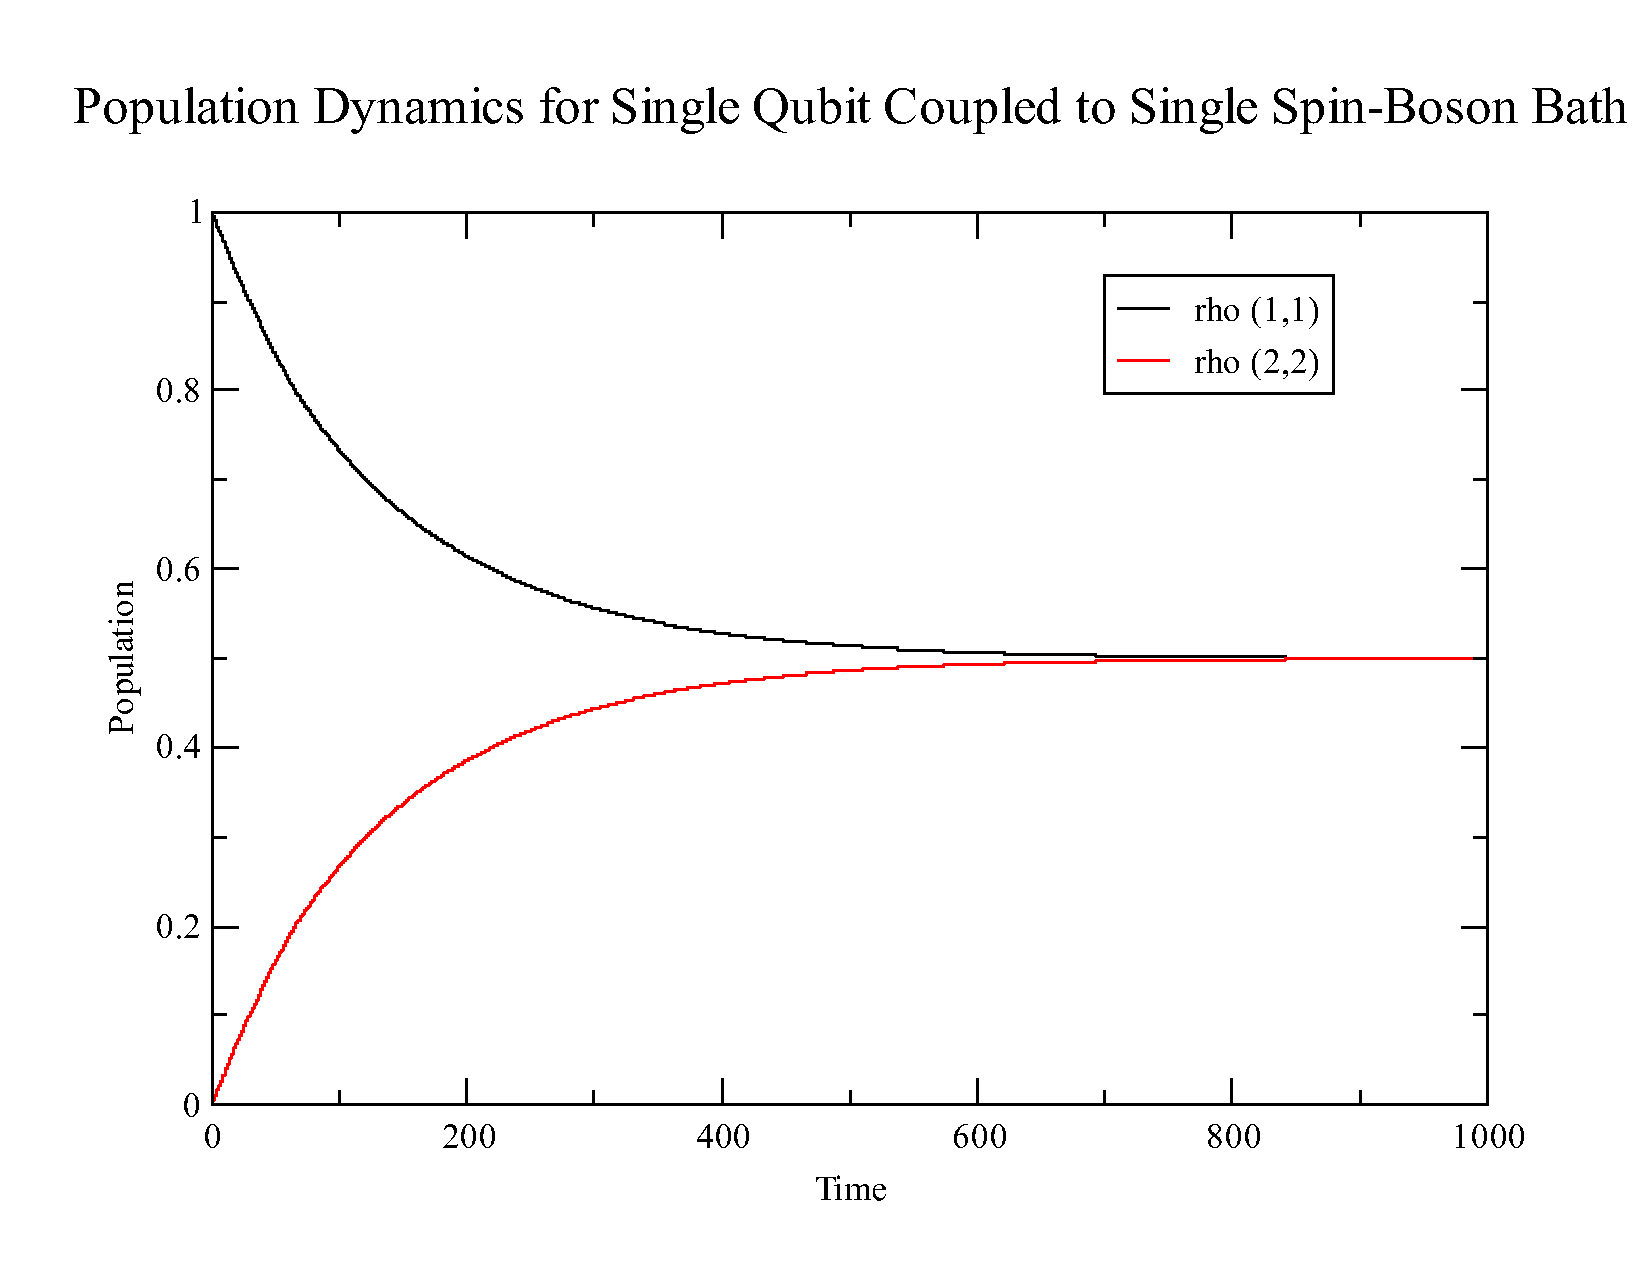
\includegraphics[scale=0.5]{plotQ1B1.pdf}
%	\label{fig:q1b1}
%\end{figure}
%
%We next consider a system of two entangled qubits, in which a single qubit is coupled to a spin-boson bath. The Hamiltonian for the qubit system is given by $$H_0 = \frac{1}{2}\sigma_z\ten\I + \frac{1}{2}\I\ten\sigma_z + \left(\sigma^+\ten\sigma^-+\sigma^-\ten\sigma^+\right).$$The interaction between the system and the bath is mediated by $$V_I = \lambda\I\ten\sigma_x$$where we again use $\lambda=0.1$. As before, we take $T=1.0$ and $gamma=0.1$. The initial density matrix is given by
%$$rho(0) =
%\begin{pmatrix}
%0 & 0 & 0 & 0 \\
%0 & 1 & 0 & 0 \\
%0 & 0 & 0 & 0 \\
%0 & 0 & 0 & 0
%\end{pmatrix}$$
%The population dynamics are illustrated in \ref{fig:q2b2}.
%
%\begin{figure}[h]
%	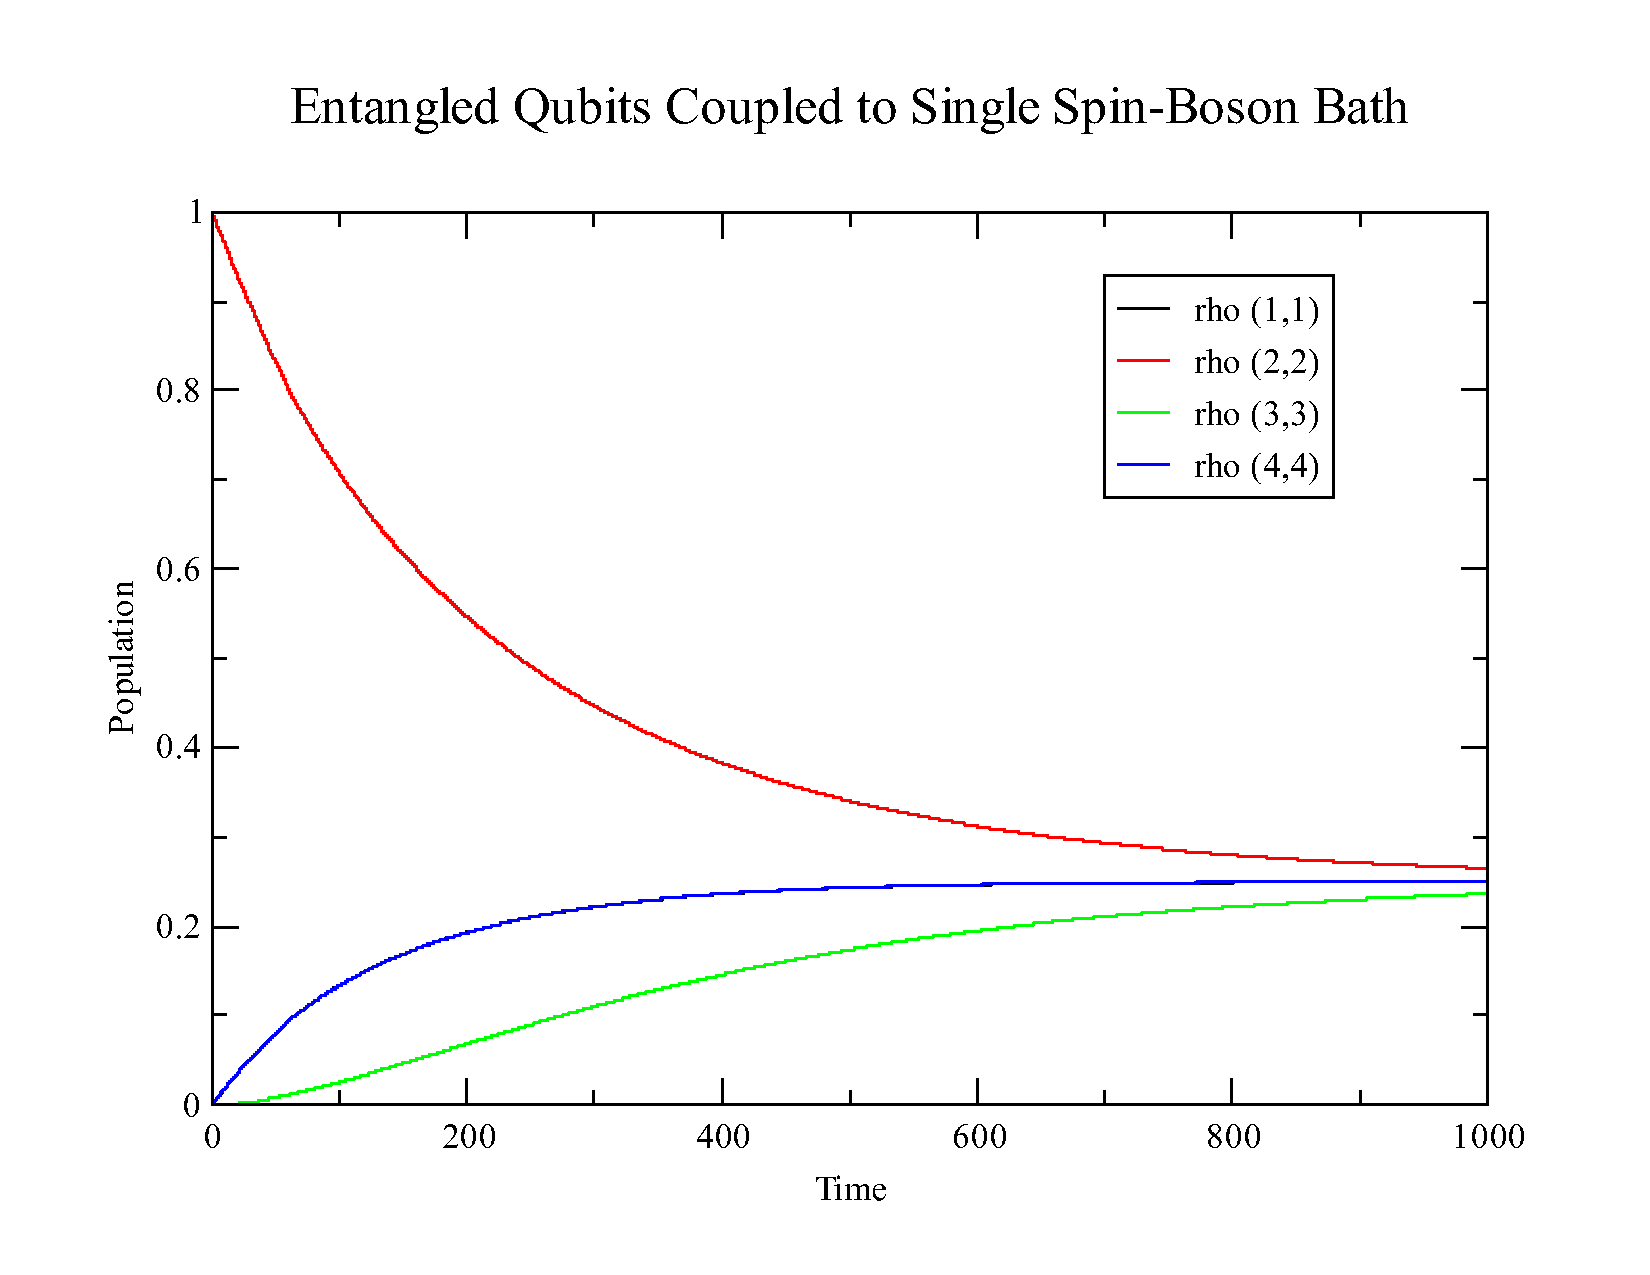
\includegraphics[scale=0.5]{plotQ2B1.pdf}
%	\label{fig:q2b2}
%\end{figure}

\end{document}
